
% Please clean this up, flesh it out, use physics package macros. Mark equations where possible.
% This is a lecture notes on differential geometry for GR taken during lecture and the instructor spoke a lot,
% but a lot of concepts or words are missing.
% but this is the gist, kindly expand upon it. It refers to the work of 
% Wald and Liang & Zhou
% % =======================================
% % MEETING 5
% % ---------------------------------------
% % DATE   - SEPTEMBER 2, 2026 
% % FORMAT - FACE TO FACE
% % =======================================
% % TOPIC  - VECTORS, TENSORS
% % =======================================

\subsection{Spacetime as a Manifold}

We consider spacetime as a differentible or smooth manifold, i.e.,
topological space that is locally $\mathbb{R}^n$

To recap, manifolds $\mcal{M}$ are objects where we can assign
to be locally $\R^n$ with charts. For instance, suppose a manifold
with a topology $\qty{Q_\alpha}$, you can represent a topology
$Q_1$ using chart $\psi_1$ to be spherical coordinates $\vb{r}= (r,\theta,\phi)$, where we limit this to be $r\neq0$,
and another topology $Q_2$ with a chart $\psi_2$ that maps it to the
coordinate system $\vb{x} = (x,y,z)$. If the two topologies intersect
at an area $Q_1 \cap Q_2$, we can then switch between the two
by composing the chart $\psi_2$ and inverse of $\psi_2$, or equivalently,
making the cartesian system a function of the spherical coordinate system and vice versa.
\begin{equation}
	\label{eq:} %kindly name this
	\vb{x}(\vb r) = \psi_1 \circ \psi_2\inv
\end{equation}
\begin{equation}
	\label{eq:} %kindly name this
	\vb{r}(\vb x) = \psi_2 \circ \psi_1\inv
\end{equation}


\begin{figure}[h]
    \centering
    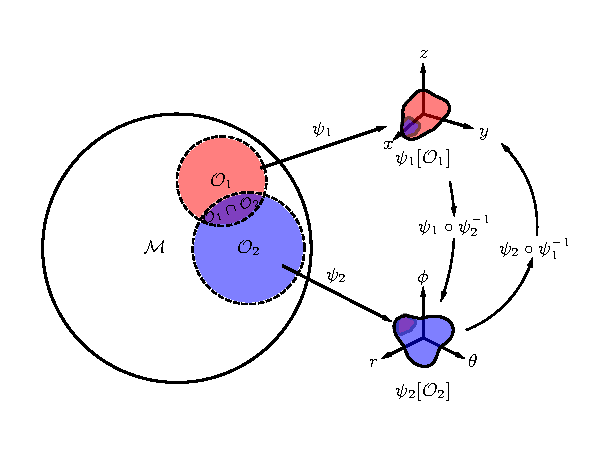
\includegraphics[width=4in, height = 3in]{images/manifold_example.pdf}
    \caption{An example of manifold being represented in differnt coordinate systems, and how to interchange them }
    \label{fig:} %name this
\end{figure}

The intersection is
\[
	\mcal{M} = \bigcup_\alpha Q_\alpha
\]
With chart
\[
	\qty{ Q_\alpha, \psi_\alpha }
\]

\[
	\psi_\alpha \circ \psi\inv_\beta
\]
Implies smooth / differentiable



The intersection allows us to change coordinate systems when we
encounter coordinate singularities, we simply switch to a system were
it doesn't exist.

$r=0$ in spherical is a physical singularity in GR but it is regarded as
not part of space time

\subsubsection{General Covariance}

Laws of Physics must be expressed in terms of geometric structures/objects
\begin{enumerate}[(a)]
    \item scalars
	\item vectors
	\item one forms / dual vectors
	\item tensors
	\item spinors (doesnt sit in GR)
\end{enumerate}

\subsubsection{Scalar}

A scalar function is defined as
\begin{equation}
	\label{eq:}
	f: \mcal{M}\to \R^n
\end{equation}
that is, a mapping of the manifold to the real numbers. We take a topology
on $\mcal M$, p, that is homeomorphic to $\R^n$ via a chart $\psi$.

no coordinate system! (simply assigning numbers to points in space time)
We then assign values to points
\[
	f: p\mapsto f(p) \in \R
\]

\[
	f\circ \psi\inv: R^\mu \to \R
\]
\[
	\vb{x}\mapsto f\circ\psi\inv = f(\vb{x})
\]
\begin{figure}[h]
    \centering
    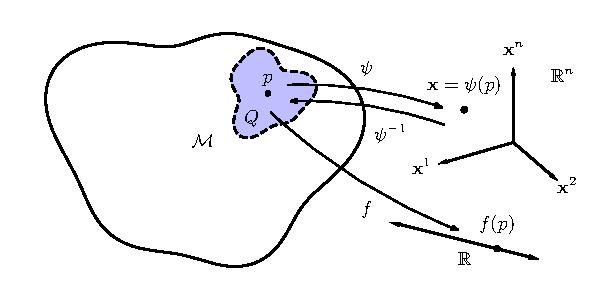
\includegraphics[width=3in]{images/manifoldtoscalar}
    \caption{Manifolds to scalar functions}
    \label{fig:}
\end{figure}

Chart coord/rep of the function
\[
	\vb{x} \equiv (x^1,x^2,...,x^n)
\]
ONly position vector in $\R^n$

To be able for this manifold to be differentiable, we
need the above chart.

If $f(\vb{X})$ is continously differentiable, then it is said to be smooth
\[
	f(\vb x)\equiv C^\infty (\mcal M) \text{ or } \mcal F(\mcal{M})
\]
-- set of smooth functions in a manifold


\[
	x^\alpha (p) \equiv \psi^\alpha, (p)
\]
coordinate scalars / functions

\subsubsection{Vectors}

Suppose a cartesian basis $x_1, x_2, x_3$. Suppose points $p$ and $q$.
Suppose a line pointing from $p$ to $q$, call it $\overline q$.

In R^3, pq is an affine structrue. Howeverm this doesn't apply in R^n
(define what is an affine structure)

\begin{figure}[h]
    \centering
    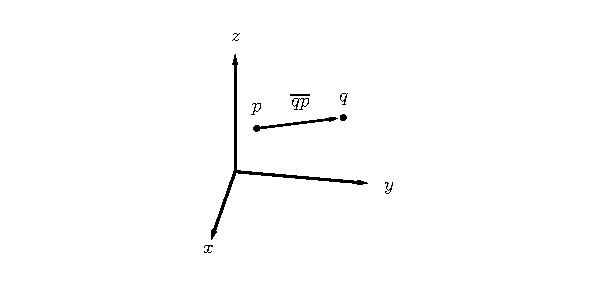
\includegraphics[width=4in,heit 3in]{images/R3vectors.pdf}
    \caption{} %add
    \label{fig:} %add
\end{figure}

A vector is in a linear vector space \bb{V} (algebraraic object) (rules of combining objects)

can still be summed which still produce a vector (closuer)
\[
	\alpha \vb{v}_1 + \beta \vb{v}_2 \in \bb{V}
\]

if $\vb{v}_1,\vb{v}_2\in\bb{V}$ , $\alpha,\beta\in\R$

Anything can be a vector, as long as it satisfies all the properties of a vector.

ONe generalizes the notion of a vector in \R^3 to general manifolds using the idea of a
\textit{directional derivative}


\[
	\vb{v}_p(f) \equiv \lim_{t\to0} \frac{f(\vb{x}_p + t\vb{v}_p) - f(\vb{x}_p)}{t}
	\equiv \vb{v}_p \cdot \grad f
\]

ONly works in R^3 or R^n due to pisitional vectors (\vqb{x}_p)

We need to change this so that we wouldn't need affine structures.

In R^3

\begin{enumerate}[(1)]
    \item Linearity
		\[
			\vb{v}_p (\alpha f + \beta g) = \alpha \vb{v}_p(f) + \beta \vb{v}_p(g)
		\]
		\alpha, \beta \in R
		f,g \in \mcal{F}(\R^n)
		
	\item Leibniz Property
		\[
			\vb{v}_p (fg) = f(p) \vb{v}_p(g) + g(p) \vb{v}_p (f)
		\]
		(\alpha \vb{v}_p + \beta\vb{w}_p)(f)
		(\alpha \vb{v}_p + \beta \vb{w}_rp)\cdot \grad f
\end{enumerate}

We define the above to manifolds such that the mapping
\[
	\vb{v}_p : \mcaL{F}\to\R^n
\]
functions to real numbers is a vector that satisfies (1) and (2)


Where is the arrow? Arrow are the preconcieved notions of vectors, why dont it
appear here?

\begin{theorem}{Vectors}
	The set of all vectors $\vb{v}_p$ at $p\in\mcal M$ is a vector space
	$T_p M$ \footnote{Tangent space at $p$}
\end{theorem}

\begin{proof}
	(a)
    Define $+$
	\[
		(\vb{v}_p + \vb{w}_p) (f) := \vb{v}_p(f) + \vb{w}_p (f)
	\]
	\[
		(\alpha \vb{v}_p) (f) = \alpha (\vb{v}_p (f))
	\]
	\[
		\vb{0}(f) = 0
	\]
	(b)
	We use these to prove the theorem
	\[
		(\alpha \vb{v}_p + \beta \vb{w}_p)(f)
	\]
	show that the result is a vector(closure and leubniz)
\end{proof}

All vectors in vector space is from the origin.
which is different from vectors in \R^n


Given a chart $\{x^\mu\}$ on $\mcal M$

we define
\[
	(\partial_\mu)_p f := \eval{\pdv{f\circ\psi\inv}{x^\mu}}_{\psi(p)}
\]

\partial_n are maps in functions , p are n-vectors, and f\circ\psi\inv
is a coord rep in \R^n

A vector is nothing but a derivative operator.

The definition is a basis for TpM

\begin{figure}[h]
    \centering
    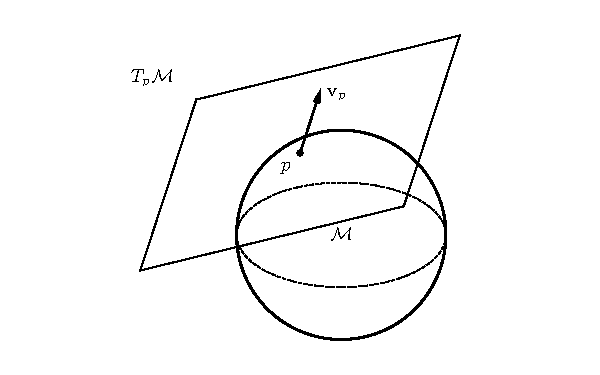
\includegraphics[width=3in]{images/vectordef.pdf}
    \caption{A vector as a basis of a manifold}
    \label{fig:}
\end{figure}

Then,
\[
	(\partial_\mu)_p := \eval{\pdv{f(x^{-\mu})}{x\mu}}_{x_p}
\]

\begin{theorem}{}  % name this
	Given a chart $\{x^\mu\}$ the set of vectors $\qty{\partial_mp}$
	constitute a basis for TpM
\end{theorem}

\begin{proof}
	(1) Linear independence
	\[
		\alpha^\mu \partial_\mu = \vb{0}
	\]
	\[
		\implies \alpha^\mu = 0
	\]
	\[
		(\alpha^\mu\partial_mu)(f) = \vb{0}(f)
		= 0
	\]
	\[
		(\alpha^\mu \partial_mu)(x^\nu) = 0
		\implies\alphaa^\mu(\partial_mu x^nu) = 0
		\implies
		(\partial_\mu) x^\nu := \pdv{(\psi^nu\circ \psi\inv)^\nu}{x^\mu} \\
		&=
		\pdv{x^\nu(x^{-\mu})}{x^mu}\big|_{x_p}
		&= \pdv{x^nu}{x^mu} = \tensor{\delta}^{^\nu_\mu}
	\]
	Then
	\[
		\alpa^\nu =\alpha^{mu}\delta^\nu_mu = 0
	\]
	(2) Spanning (Wald p.16)
	Show that $v_p\in T_p M$
	\[
		v_p = v^\mu(\partial_nu)_p\\
		v^\nu = v_p (x^nu)
	\]

	Abstract index notation
	v^\alpha : vector itself

	Then the arrow is
	\[
		\vb{v} &= v^\mu \partial_\mu\\
			   &= v^x \pdv{}{x} + v^y \pdv{}{y} + v^z  \pdv{}{z} 
			   &= v^r \pdv{}{r} + v^\theta \pdv{}{\theta} + v^\phi  \pdv{}{\phi} 
	\]
	
\end{proof}

